% !TEX root = ./paper/paper.tex
%% This is an abbreviated template from http://www.sigplan.org/Resources/Author/.

\documentclass[acmsmall,review,nonacm]{acmart}

\usepackage{amsthm}
\usepackage{graphicx} % Required for inserting images
\usepackage{amsmath}
\usepackage{xcolor}
\usepackage{listings}
\usepackage{mathpartir} % For inference rules
\usepackage{stmaryrd}   % For semantics brackets
\usepackage{tikz}
\usepackage[utf8]{inputenc}
\usepackage{tikzpeople} % Included to prevent conflicts
\usetikzlibrary{positioning,arrows.meta}

\definecolor{predblue}{RGB}{100, 100, 255}
\definecolor{validgreen}{RGB}{0, 255, 0}
\definecolor{invalidred}{RGB}{255, 0, 0}

\newtheorem{definition}{Definition}
\newtheorem{theorem}{Theorem}
\newtheorem{lemma}{Lemma}
\newtheorem{hypothesis}{Hypothesis}

% Helper for inference rules
\newcommand{\infrule}[2]{\frac{\displaystyle #1}{\displaystyle #2}}


\begin{document}

%%
%% The "title" command has an optional parameter,
%% allowing the author to define a "short title" to be used in page headers.
\title{Skja: Adversarial Logic on Steroids}

%%
%% The "author" command and its associated commands are used to define
%% the authors and their affiliations.
%% Of note is the shared affiliation of the first two authors, and the
%% "authornote" and "authornotemark" commands
%% used to denote shared contribution to the research.
\author{Aka Sai Lalith Kumar}
\email{sailalithkumar.aka@colorado.edu}
\affiliation{%
  \institution{University of Colorado Boulder}
  \country{USA}
}


%%
%% The abstract is a short summary of the work to be presented in the
%% article.
\begin{abstract}
We introduce \textit{Skja}, a new incorrectness logic \cite{o2019incorrectness} which extends on \textit{Adversarial Logic} \cite{vanegue2022adversarial} with spi-calculus. Adversarial logic is very interesting in that it lets you apply under-approximation for exploitability analysis. The current core limitation of adversarial logic is that it only allows for parallel composition over multiple programs but it has problems with the model. With Skja, we bring the rich theory of spi-calculus to let the logic be composable for any infinite arbitrary set of  programs which may be adversarial or not. This lets us encode and talk about attacks like Man-in-the-middle (MiTM) attacks and DDoS (Denial of Service) attacks. For this end, we first prove that parallel composition is a monoid over the adversarial logic grammar. We change the denotational semantics and program rules to support n-ary parallel composition while also proving that the changes do not effect the soundness. We also show.
 \end{abstract}

%%
%% This command processes the author and affiliation and title
%% information and builds the first part of the formatted document.
\maketitle

\section{Introduction}
When one reasons about programmes, we have access to a rich variety of logics, and one of them would be incorrectness logic \cite{o2019incorrectness} which is equivalent to \cite{de2011reverse}. The logic targets under-approximating the post of a condition c; this is symmetrical to the work done by Hoare\cite{hoare1969axiomatic} which over-approximates. 
The way we can understand this through diagrammatic representation is by visualising the state space as a hierarchy of set inclusions, taken from O'Hearn's presentation. 
As shown in Figure \ref{fig:logic_triangle}, the central arrow represents the \textit{strongest postcondition} ($post(c)$), which describes exactly the set of states reachable by the program.

\begin{figure}[h]
    \centering
    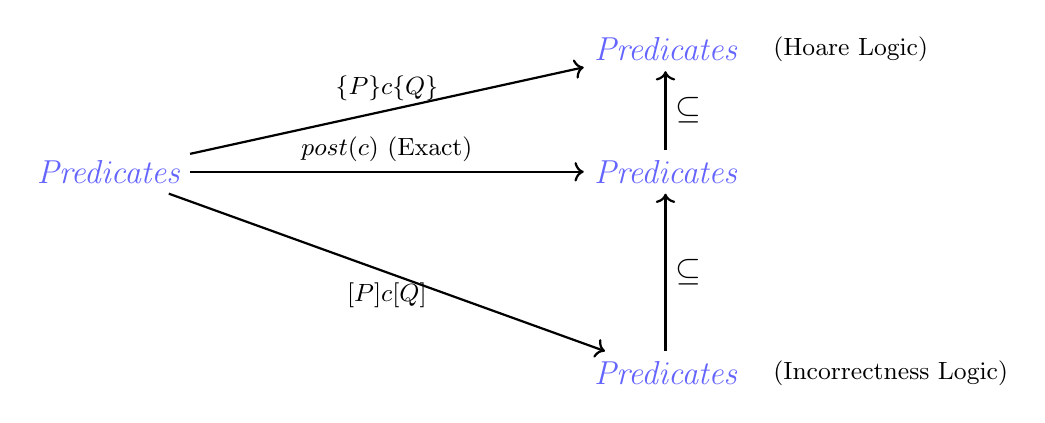
\begin{tikzpicture}[
        node distance=2cm,
        text=predblue, 
        font=\large\itshape,
        thick
    ]
        % Nodes
        \node (start) {Predicates};
        
        \node[right=5cm of start] (mid) {Predicates};
        \node[above=1cm of mid] (top) {Predicates};
        \node[below=2cm of mid] (bot) {Predicates};

        % Arrows from Start
        \draw[->] (start) -- (top) node[midway, above, text=black, font=\small] {$\{P\}c\{Q\}$ };
        \draw[->] (start) -- (mid) node[midway, above, text=black, font=\small] {$post(c)$ (Exact)};
        \draw[->] (start) -- (bot) node[midway, below, text=black, font=\small] {$[P]c[Q]$ };

        % Vertical Inclusions
        % The Top (Over) is a SUPERSET of the Middle (Exact)
        \draw[->] (mid) -- (top) node[midway, right, text=black, font=\large] {$\subseteq$};
        
        % The Bottom (Under) is a SUBSET of the Middle (Exact)
        \draw[->] (bot) -- (mid) node[midway, right, text=black, font=\large] {$\subseteq$};
        
        % Labeling the logic types
        \node[right=0.2cm of top, text=black, font=\small] {(Hoare Logic)};
        \node[right=0.2cm of bot, text=black, font=\small] {(Incorrectness Logic)};

    \end{tikzpicture}
    \caption{The hierarchy of program logic. Hoare logic (top) over-approximates the reachable states, while Incorrectness logic (bottom) under-approximates them.}
    \label{fig:logic_triangle}
\end{figure}

In this hierarchy, the top layer corresponds to standard Hoare Logic. It provides an \textit{over-approximation}, meaning the postcondition $Q$ must contain all reachable states ($post(c) \subseteq Q$). This is useful for proving safety (i.e., "nothing bad happens").

Conversely, the bottom layer represents under-approximation. Here, the postcondition $Q$ must be a \textit{subset} of the reachable states ($Q \subseteq post(c)$). This logic is useful for proving the existence of bugs or specific reachable states (i.e., "something bad definitely happens").
Now, you can also observe, the triangle for top is rather short compared to the triangle for the bottom. This is a delibrate choice to highlight the fact that over-approximation enojoyed 5 decades of being in the front seat \cite{apt1981ten,apt1983ten,ali2017survey} and hence the closeness to the prefect postcondition.

To show case an example with under-approximation, we take a rather simple looking but tricky example derived from \cite{de2011reverse} below comparing the validity of the triplets shown below:

\begin{equation*}
    \langle T \rangle \quad x := y; \ z := x \quad \langle z = y \rangle \quad \colorbox{invalidred}{\textbf{Not Valid}}
\end{equation*}

This triplet is invalid in under-approximation logic. While it is true that $z=y$ in the final state, the assertion $\langle z = y \rangle$ as a set includes states where $x \neq y$ (e.g., state $\{x=0, z=1, y=1\}$). However, the program guarantees $x=y$. Because the assertion includes "extra" states that the program logic cannot reach, it is not a valid subset (under-approximation) of the true postcondition.

\begin{equation*}
    \langle T \rangle \quad x := y; \ z := x \quad \langle z = y \land x = y \rangle \quad \colorbox{validgreen}{\textbf{Valid}}
\end{equation*}

This triplet is valid. By conjoining $x=y$, we restrict the postcondition to exclude the unreachable states. The resulting set matches exactly the behavior of the code, satisfying the requirement $Q \subseteq post(c)$.
Application of under-approximation to security reasoning is a very novel yet fundamental contribution \cite{vanegue2022adversarial}.
And this contribution brings proving software or protocols are secure to the realm of finding bugs or vulnerabilities aka exploitability analysis \cite{elder2024survey}.
A simple analysis tool running on a rather not complicated software usually returns many bugs \cite{serebryany2016continuous} and many of them are usually false positives.
In the era of move fast, break fast \cite{cohen2004introduction} this puts a lot of burden on security bug triagers who have to classify each bug for it's true validty and slows the development cycle a lot given if a team moves with an unsure bug.
This breaks rythm and destroys planning of the required

\section{Overview}

\section{New Semantics}

In this section we build all the semantics and rules which transform adversarial logic to Skja.
First, we assume the reader is familiar with the semantics of adversarial logic and refer them to the original paper for the full set \cite{vanegue2022adversarial}, our work states what is new to the established semantics.  

First we change the state space. In AL, states were rigid couples $(\sigma_p, \sigma_a)$. To support $n$-ary composition, we map Process IDs to their local stores.

\begin{definition}[General State Space]
$\Sigma ::= [PIDs \rightharpoonup Variables \to Values]$
\end{definition}

Let $\Pi \in \Sigma$ be a global state. We denote $\Pi(i)$ as the local store of process $i$.
We also maintain the global channel state $\Gamma \in [Channels \to List(Values)]$. A configuration is a tuple $\langle \Pi, \Gamma \rangle$.

A key notation change from adversarial logic is that instead of using $[\epsilon:P]$ where $\epsilon \in \{ad, ok\}$, we define $\Delta$ as a mapping from PIDs to assertions.

\begin{definition} [Generalized Triple]
    $[\Delta_{pre}] C [\Delta_{post}]$
\end{definition}


For processes Alice ($A$), Bob ($B$), and Eve ($E$), $\Delta$ maps identities to assertions: $\{A: P_A, B: P_B, E: P_{Eve}\}$.
The triple $[\Delta] C [\Delta']$ is valid if, for all processes $i \in dom(\Delta)$, the local execution satisfies the under-approximate relation between $\Delta(i)$ and $\Delta'(i)$.

\subsection{Syntax of Assertions}
To reason about what an adversary knows, we define the syntax for expressions and assertions, adapting the model from \cite{vanegue2022adversarial}.

\begin{definition}[Syntax]
\begin{align*}
    Variables \ V &::= x \mid n \mid \alpha \\
    Expressions \ E &::= V \mid rand() \mid \text{enc}(E, K) \mid \langle E, E \rangle \\
    Assertions \ P, Q &::= E = E \mid \text{Knows}(E) \mid P \land Q \mid \exists x. P
\end{align*}
\end{definition}
Here, $\text{Knows}(E)$ is a predicate indicating that the value $E$ is derivable from the agent's current knowledge set using Dolev-Yao deduction rules.

\subsection{Semantics}
\begin{definition} [Small-step semantics for Composition]
Let $C_1 \parallel \dots \parallel C_n$ be a composition of $n$ processes.
\begin{itemize}
    \item \textbf{Independent Step:} If process $i$ takes a local step $\langle \sigma_i, \Gamma \rangle \to \langle \sigma_i', \Gamma \rangle$, then:
    $$ \langle \Pi[i \mapsto \sigma_i], \Gamma \rangle \to \langle \Pi[i \mapsto \sigma_i'], \Gamma \rangle $$
    \item \textbf{Communication Step:} If process $i$ writes to channel $c$ and process $j$ reads from channel $c$, they synchronize:
    $$ \langle \Pi, \Gamma \rangle \xrightarrow{i!c(v), j?c(v)} \langle \Pi', \Gamma' \rangle $$
    where $\Pi'$ updates the local variables of $i$ and $j$ appropriately.
    \item \textbf{Termination:} $skip \parallel \dots \parallel skip$ is the terminal configuration.
\end{itemize}
\end{definition}

We restate the properties of channels and local variables for processes from adversarial logic.
\begin{hypothesis}[Ownership Principle]
\leavevmode
    \begin{itemize}
        \item No two parallel processes share the same local variables and are distinctly separated (Disjointness). $\forall i \neq j, dom(\Pi(i)) \cap dom(\Pi(j)) = \emptyset$.
        \item They can only communicate through channels, which we state are global and represented by $\Gamma$.
    \end{itemize}
\end{hypothesis}

\subsection{Inference Rules}
To support the $n$-ary composition defined above, we extend the rules of adversarial logic by modifying the 

\textbf{1. The n-Par Rule.} 
This rule allows us to combine independent proofs of $n$ processes. It relies on the disjointness hypothesis.

$$
\inferrule*[lab=n-Par]
{ \forall i \in \{1..n\}, \quad [\Delta_{pre}(i)] C_i [\Delta_{post}(i)] }
{ [\Delta_{pre}] C_1 \parallel \dots \parallel C_n [\Delta_{post}] }
$$

\textbf{2. The n-Com Rule.} 
This is the workhorse of protocol verification when it comes to Skja. It synchronizes a sender $i$ and a receiver $j$ over channel $c$. Other processes $k$ remain idle (frame property).

$$
\inferrule*[lab=n-Com]
{ 
[\Delta_{pre}(i)] \text{out}(c, v) [\Delta_{post}(i)] \\
  [\Delta_{pre}(j)] \text{in}(c, x) [\Delta_{post}(j)] \\
  \forall k \notin \{i, j\}, \Delta_{pre}(k) = \Delta_{post}(k) }
{ [\Delta_{pre}] \left( \dots \parallel \text{out}_i \parallel \dots \parallel \text{in}_j \parallel \dots \right) [\Delta_{post}] }
$$

Semantically, this implies a logical flow of the value $v$ from $i$ to $j$:
$$ \exists v, (\Delta_{pre}(i) \implies x=v) \land (\Delta_{post}(j) \implies x=v) $$
\subsection{The Dolev-Yao Adversary Model}
To reason about protocols, we adopt the standard Dolev-Yao model, assuming the network is under total control of the adversary. The adversary can read, block, and modify messages but cannot break cryptography without the correct keys.

We formalize the attacker's capabilities using the deduction relation $\vdash$. Let $\mathcal{K}$ be the set of messages currently known to the attacker. The relation $\mathcal{K} \vdash m$ (read: "from knowledge $\mathcal{K}$, message $m$ can be derived") is defined inductively:

\begin{gather*}
\infrule{m \in \mathcal{K}}{\mathcal{K} \vdash m} \text{(Axiom)} \quad
\infrule{\mathcal{K} \vdash m_1 \quad \mathcal{K} \vdash m_2}{\mathcal{K} \vdash \langle m_1, m_2 \rangle} \text{(Pairing)} \quad
\infrule{\mathcal{K} \vdash \langle m_1, m_2 \rangle}{\mathcal{K} \vdash m_i} \text{(Proj)}
\\[2ex]
\infrule{\mathcal{K} \vdash m \quad \mathcal{K} \vdash k}{\mathcal{K} \vdash \{m\}_k} \text{(Encrypt)} \qquad
\infrule{\mathcal{K} \vdash \{m\}_k \quad \mathcal{K} \vdash k^{-1}}{\mathcal{K} \vdash m} \text{(Decrypt)}
\end{gather*}

In Skja, this deduction relation connects the operational semantics to the assertion logic. We define the semantics of the assertion $\text{Knows}(m)$ as follows:
$$ \sigma \models \text{Knows}(m) \iff \sigma(\text{knowledge}) \vdash m $$
This definition is crucial for under-approximation. Unlike safety verification, where one must compute the potentially infinite set of all derivable knowledge to prove a secret is \textit{never} leaked, Skja only requires demonstrating the existence of a single derivation tree. If there exists a sequence of rule applications allowing the adversary to construct the message $m$ needed for the next step of the attack trace, the assertion holds. This makes the check constructive and efficient for exploit generation.


\section{Proofs}

\subsection{Proof of Composition (||) forms a monoid}

The reason we would like to have composition as a commutative monoid is that it frees us from thinking about ordering and composition of operators, allowing us to treat the system as a "soup" of processes, consistent with the chemical abstract machine model often used for process calculi.

First, we define the structural congruence relation ($\equiv$) for our logic. This relation identifies process terms that are syntactically different but semantically identical.

\begin{definition}[Structural Congruence]
The parallel composition operator $\parallel$ satisfies the following laws:
\begin{align}
    P \parallel Q &\equiv Q \parallel P & \text{(Commutativity)} \\
    (P \parallel Q) \parallel R &\equiv P \parallel (Q \parallel R) & \text{(Associativity)} \\
    P \parallel skip &\equiv P & \text{(Identity)}
\end{align}
\end{definition}

\begin{theorem}
    (Process, ||, skip) form a commutative monoid.
\end{theorem}

Proof: A commutative monoid has three properties for it to satisfy. We show that (||) satisfies all below:
\begin{itemize}
    \item \textbf{Commutativity:} For some processes P and Q, $P \parallel Q \equiv Q \parallel P$.
     Every derivation of a step from $P \parallel Q$ is obtained by applying one of the small-step rules. Swapping the syntactic positions of P and Q gives a derivation of the same step from $Q \parallel P$ (process IDs are intrinsic to the state, not the syntactic position). Therefore the sets of possible traces are identical.
    
    \item \textbf{Associativity:} For some processes P, Q and R, $(P \parallel Q) \parallel R \equiv P \parallel (Q \parallel R)$.
    The transition relation is defined on the set of PIDs. Grouping $(P \parallel Q)$ is merely syntactic sugar for a set of processes $\{P, Q\}$. The execution semantics operate on the union of disjoint heaps. Since set union is associative, the composition is associative.

    \item \textbf{Identity:} For some process P, $(P \parallel skip) \equiv P$.
    The $skip$ process has no transitions and modifies no state. Its interleaving with $P$ adds no new traces and restricts no existing traces of $P$.
\end{itemize}

\begin{lemma} [Permutations of || ]
    For any set of processes $\{C_1, ..., C_n\}$, any syntactic permutation of their composition results in an equivalent system under the defined denotational semantics.
\end{lemma}


\subsection{Soundness}
We prove the soundness of the inference rules by showing that if the premises hold, the conclusion satisfies the under-approximation reachability property (Lemma 2).

\begin{lemma}[Characterization for n-ary Systems]
The triple $[\Delta_{pre}] C [\Delta_{post}]$ is true iff every state in $\llbracket \Delta_{post} \rrbracket$ is reachable from a state in $\llbracket \Delta_{pre} \rrbracket$ via the operational semantics of $C$.
\end{lemma}

\begin{theorem}[Soundness of n-Par]
The n-Par rule is valid.
\end{theorem}
\begin{proof}
Let $\Pi' \in \llbracket \Delta_{post} \rrbracket$ be a target global state. By the definition of the state space, $\Pi'$ decomposes into local stores $\Pi'(i)$. From the premises, for each $i$, $[\Delta_{pre}(i)] C_i [\Delta_{post}(i)]$ is valid, implying $\exists \sigma_i \in \llbracket \Delta_{pre}(i) \rrbracket$ such that $\sigma_i \to^* \sigma_i'$ via $C_i$.
By the \textbf{Ownership Principle} (Hypothesis 1), domains are disjoint. Consequently, the \textbf{Independent Step} semantics apply, allowing local transitions to be interleaved without interference. Thus, starting from $\Pi = \bigcup_i \sigma_i$, the global system reaches $\Pi'$ via $C_1 \parallel \dots \parallel C_n$.
\end{proof}

\begin{theorem}[Soundness of n-Com]
The n-Com rule is valid.
\end{theorem}
\begin{proof}
Let $\Pi' \in \llbracket \Delta_{post} \rrbracket$. For idle processes $k \notin \{i,j\}$, $\Delta_{pre}(k) = \Delta_{post}(k)$, satisfying the frame property via trivial reachability (0 steps).
For interacting processes, the premises guarantee the existence of local pre-states $\sigma_i \in \llbracket \Delta_{pre}(i) \rrbracket$ and $\sigma_j \in \llbracket \Delta_{pre}(j) \rrbracket$ that can perform output and input respectively.
The \textbf{Communication Step} semantics $\langle \Pi, \Gamma \rangle \xrightarrow{i!c(v), j?c(v)} \langle \Pi', \Gamma' \rangle$ synchronizes these steps. Specifically, the semantic rule updates the receiver's store $\sigma_j'$ such that $x = v$. Since the premises hold and the operational semantics explicitly enforce the data flow $v \to x$, the global post-state where receiver variable $x$ holds sender value $v$ is reachable from $[\Delta_{pre}]$.
\end{proof}


\section{Reasoning with Sjka: Needham-Schroder}

\subsection{Needham-Schroder}
Needham-Schroder(NS)\cite{needham1978using}, is an authenatication protocol. The way it runs is as follows:
\begin{figure}
    \centering
    \label{fig:ns}
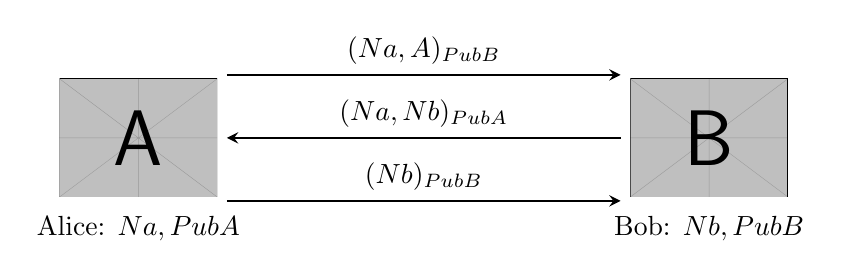
\begin{tikzpicture}[>=stealth]
\node[label=below:{Alice: $Na, PubA$}] (A) {\includegraphics[width=2cm,keepaspectratio]{example-image-a}};
\node[right=5cm of A, label=below:{Bob: $Nb, PubB$}] (B) {\includegraphics[width=2cm,keepaspectratio]{example-image-b}};

\draw[->,thick] ([yshift=8mm]A.east) -- node[above]{$(Na, A)_{PubB}$} ([yshift=8mm]B.west);
\draw[<-,thick] (A.east) -- node[above]{$(Na, Nb)_{PubA}$} (B.west);
\draw[->,thick] ([yshift=-8mm]A.east) -- node[above]{$(Nb)_{PubB}$} ([yshift=-8mm]B.west);
\end{tikzpicture}
    \caption{Needham-Schroder}
\end{figure}


\begin{figure}[h!]
\centering
\tikzset{
  stepnum/.style={circle, draw, inner sep=1.5pt, font=\small, fill=white}
}

\begin{tikzpicture}[>=stealth]

% --- NODES for Participants ---
% Spacing is kept at the more compact 3.5cm
\node (A_img) {\includegraphics[width=2cm,keepaspectratio]{example-image-a}};
\node[right=3.5cm of A_img] (M_img) {\includegraphics[width=2cm,keepaspectratio]{example-image-c}};
\node[right=3.5cm of M_img] (B_img) {\includegraphics[width=2cm,keepaspectratio]{example-image-b}};

% --- Labels ---
% Changed "Mallory" to "Charlie" and "PubM" to "PubC"
\node[above=0.2cm of A_img] {Alice};
\node[below=0.2cm of A_img] {$Na, PubA$};
\node[above=0.2cm of M_img] {Charlie (Attacker)};
\node[below=0.2cm of M_img] {$PubC$};
\node[above=0.2cm of B_img] {Bob};
\node[below=0.2cm of B_img] {$Nb, PubB$};

% --- MESSAGE FLOWS ---
% Removed 'dashed' from arrows and updated keys to PubC

% 1. Alice -> Charlie -> Bob (Initiation)
\draw[->, thick] ([yshift=8mm]A_img.east) --
    node[above,midway] {$(Na, A)_{PubC}$} % Key changed
    node[stepnum,pos=0.1,above=1pt] {1}
    ([yshift=8mm]M_img.west);
    
\draw[->, thick] ([yshift=8mm]M_img.east) -- % REMOVED dashed
    node[above,midway] {$(Na, A)_{PubB}$}
    node[stepnum,pos=0.1,above=1pt] {2}
    ([yshift=8mm]B_img.west);

% 2. Bob -> Charlie -> Alice (Response)
\draw[<-, thick] (M_img.east) -- % REMOVED dashed
    node[above,midway] {$(Na, Nb)_{PubA}$}
    node[stepnum,pos=0.9,above=1pt] {3}
    (B_img.west);
    
\draw[<-, thick] (A_img.east) --
    node[above,midway] {$(Na, Nb)_{PubA}$}
    node[stepnum,pos=0.9,above=1pt] {4}
    (M_img.west);

% 3. Alice -> Charlie -> Bob (Confirmation)
\draw[->, thick] ([yshift=-8mm]A_img.east) --
    node[below,midway] {$(Nb)_{PubC}$} % Key changed
    node[stepnum,pos=0.1,below=1pt] {5}
    ([yshift=-8mm]M_img.west);
    
\draw[->, thick] ([yshift=-8mm]M_img.east) -- % REMOVED dashed
    node[below,midway] {$(Nb)_{PubB}$}
    node[stepnum,pos=0.1,below=1pt] {6}
    ([yshift=-8mm]B_img.west);

\end{tikzpicture}
\caption{Lowe's man-in-the-middle attack, where Charlie impersonates Alice.}
\end{figure}


We refer to figure 1, which shows the steps of NS protocol. First we see Alice initiating the protocol with Bob by sending here Nonce Na with her own ID paired together. This is done to make sure Bob knows who he is communicating with. Now, we see Bob responds to Alice with his own Nonce Nb and Na paired together; this is done so that Alice can confirm her nonce and ensure she is not talking to another third party, as only Bob can deduce her nonce. Now, finally, Alice sends back Bob's nonce in the same spirit as above.

This protocol is very sensible but hides a cunning attack in plain sight. We refer the reader to figure 2 for Lowe's attack. Here you see, Charlie is an impersonator. Who can be called a Dolev-Yao adversary as the semantics and powers of the same are defined in the section 2. To recap, he can replay messages, stop messages and forward them and strip messages if they're encrypted with his private key. Now in Lowe's attack, the security guarantees of Alice are maintained, meaning that they won't share the nonce with some other person who they don't know they are talking to, but for Bob it's broken.
This can be observed at the end of the protocol run where Bob thinks he is talking to Alice, but it's actually Charlie who now has Bob's and Alice's nonce, so Charlie can act as Alice and keep the conversation going. This is a failure of authentication.
\subsection{Formalizing the Attack in Skja}
We demonstrate the validity of Lowe's attack by tracing the evolution of the generalized assertion map $\Delta$ through the application of the \textbf{n-Com} rule. 

Let the initial state be $\Delta_0$. The participants have the following initial knowledge:
$$ \Delta_0 = \{ A: \text{Knows}(Na, PrivA), \ B: \text{Knows}(Nb, PrivB), \ C: \text{Knows}(PrivC) \} $$

\textbf{Phase 1: Initiation and Impersonation (Steps 1 \& 2)} \\
Alice intends to talk to Charlie. She executes $\text{out}(c, \{Na, A\}_{PubC})$. Charlie reads from $c$. Applying \textbf{n-Com}:
$$ [\Delta_0(A)] \text{out} \dots \parallel \text{in} [\Delta_1(C)] $$
The synchronization ensures the value flows to Charlie. Since Charlie possesses $PrivC$, he decrypts the message.
$$ \Delta_1(C) \implies \text{Knows}(Na) $$
Using this new knowledge, Charlie impersonates Alice. He constructs $\{Na, A\}_{PubB}$ and sends it to Bob. Applying \textbf{n-Com} between Charlie and Bob:
$$ \Delta_2(B) \implies \text{Received}(\{Na, A\}_{PubB}) $$
Bob decrypts this. Crucially, Bob's internal state now asserts he is communicating with Alice.

\textbf{Phase 2: The Oracle Step (Steps 3 \& 4)} \\
Bob responds to the perceived initiator. He sends $\{Na, Nb\}_{PubA}$. Charlie intercepts this via \textbf{n-Com}.
$$ \Delta_3(C) \implies \text{Knows}(\{Na, Nb\}_{PubA}) $$
At this stage, Charlie \textit{cannot} decrypt the message to learn $Nb$ because he lacks $PrivA$. This is where the logic highlights the vulnerability. Charlie forwards the blob opaque to Alice (Step 4). Applying \textbf{n-Com} between Charlie and Alice:
$$ \Delta_4(A) \implies \text{Received}(\{Na, Nb\}_{PubA}) $$
Alice, believing this is a valid response from Charlie (her intended partner), decrypts it. She verifies $Na$ and learns $Nb$.

\textbf{Phase 3: The Leak (Step 5)} \\
This is the fatal step. Following the protocol, Alice confirms the session by sending $Nb$ encrypted with her partner's key ($PubC$).
$$ [\Delta_4(A)] \text{out}(c, \{Nb\}_{PubC}) \parallel \text{in}(c, x) [\Delta_5(C)] $$
Applying \textbf{n-Com}, Charlie receives $x = \{Nb\}_{PubC}$. Since $\Delta_5(C)$ includes $PrivC$:
$$ \Delta_5(C) \implies \text{Knows}(Nb) $$
The adversary has successfully extracted the secret nonce $Nb$.

\textbf{Phase 4: Completion (Step 6)} \\
Charlie re-encrypts $Nb$ with $PubB$ and sends it to Bob via \textbf{n-Com}. Bob verifies $Nb$ and completes the session.

\textbf{Conclusion} \\
The final state $\Delta_{final}$ contains a contradiction to the authentication specification:
\begin{enumerate}
    \item $\Delta_{final}(B) \implies \text{Partner} = Alice$
    \item $\Delta_{final}(C) \implies \text{Knows}(Na, Nb)$
\end{enumerate}
In Skja, the reachability of $\Delta_{final}$ where the adversary knows $Nb$ constitutes a proof of the exploit. The proof script could be more integrated to look like the reasoning of adversarial logic, but we choose to keep it focused on the rules we have defined.
\section{Related Work}
Related work in program analysis and formal verification of protocols and softwares come with a rather rich history. We stand on the shoulders of the gaints, and a small exposition in this section will never give with an $n$-ary composition model based on the spi-calculus, allowing for more complex network topologies.

\section{Conclusion}
In this paper, we adapted under-approximation logic for security and boosted its versatility by integrating techniques from the spi-calculus. We demonstrated that this extension preserves the soundness of the underlying logic through formal proofs. Finally, we applied Skja to the Needham-Schroeder protocol, formally proving the validity of the classic Man-in-the-Middle vulnerability.

\begin{acks}
I thank my advisor, Dr. Gowtham Kaki. I acknowledge Dr. Bohr-Yuh Evan Chang and Kirby Linvill for their instruction on PL. Thanks to Dakota Brayan for feedback, and Dr. Fabio Somenzi for teaching me about logic.
\end{acks}

\bibliographystyle{ACM-Reference-Format}
\bibliography{paper}
\end{document}